\documentclass[conference]{IEEEtran}
\IEEEoverridecommandlockouts
% The preceding line is only needed to identify funding in the first footnote. If that is unneeded, please comment it out.
\usepackage{cite}
\usepackage{amsmath,amssymb,amsfonts}
\usepackage{algorithmic}
\usepackage{graphicx}
\graphicspath{ {./images/} }
\usepackage{textcomp}
\usepackage{xcolor}
\usepackage{hyperref}
\def\BibTeX{{\rm B\kern-.05em{\sc i\kern-.025em b}\kern-.08em
    T\kern-.1667em\lower.7ex\hbox{E}\kern-.125emX}}

\begin{document}

\title{Evaluating Various Attention in Neural Machine Translation}
\author{\IEEEauthorblockN{\textbf{Illy Hoang}}
\IEEEauthorblockA{
University of Connecticut / USA \\
Illy.Hoang@uconn.edu}
}
\maketitle


\begin{abstract}
Neural Machine Translation (NMT) quality has significantly improved over a relatively short span of time with the growing number of proposals to address various theoretical limiting factors – one namely being the incorporation of attention layers in model implementations to support contextual readings in predictions during the decoding process. This paper evaluates the translation quality of attention-based NMT with three types of models: 1) a simple seq2seq Encoder-Decoder model that shall be utilized as a ‘control’ variable for comparisons; 2) a model that computes the attention weights and context vectors of inputted sequences with the additive algorithm proposed by Bahdanau et al.; and 3) a model similar to the former that instead makes computations based on the multiplicative algorithm proposed by Luong et al. The models are trained, validated and tested using randomly generated splits from a data set compiling numerous Spanish-English pair-phrases. They are then evaluated using the BERTScore metric to better assess token similarities between machine translations and their human-produced counterparts. A
related repository \nolinkurl{https://github.com/illydh/nmt-model/tree/main/spr24-research} is dedicated to collecting
related work.
\end{abstract}

\section{Introduction and Background}
Growing up, my native language was not reinforced on me. I heavily rely on machine translation for communication between myself and non-English language speakers. Through enrollment in foreign language courses growing up, I became fascinated in how humans develop the ability to communicate in various foreign languages and hoped for the opportunity to study this in depth. When I was sought out to create an independent study project, I saw this as my opportunity.

\par

Concurrently taking UConn's course in Artificial Intelligence (AI) piqued my interest in how the subsection of Natural Language Processing (NLP) has allowed the advancement of machine translation by utilizing neural networks (NN) and reinforcement learning methods to train models with the goal of improving NMT performance \cite{b2}. I delved into its application to Natural Language Processing (NLP) and its various and numerous contributions through research over time \cite{b1}. Although documentation of advancements in NMT research have been extensive, I wanted to take this opportunity to research attention-based models specifically (1) to get a better understanding as to the infrastructure and functionality of NMT models; as well as (2) to model a solution to a presented problem.

\par

Existing research materials proposes new mechanisms for computing attention and display accuracy ratings based on their BLEU Scores, an automated method of human evaluation for NMT \cite{b3}. However, due to rapid advancements and improvements to modeling, not much work is documented for comparisons between these models to make true evaluations of their accuracy and effectiveness. Also recent publications argue that NMT evaluation has been too reliant on BLEU as an automatic evaluation metric \cite{b5} as well as that the metric poses various implications and inconsistencies in its calculations \cite{b4}. 

\par

In my work thus far, I analyze the composition of a baseline seq2seq model constructed as a recurrent NN as well two other models that includes an attention layer in the decoding process to compute attention weights and to produce context vectors following RL procedures. One method of computation for attention is the additive algorithm proposed by Bahdanau et al. \cite{b7} and the other being the multiplicative algorithm proposed by Luong et al. \cite{b8}. These machine translations are then evaluated by a BERTScore algorithm which better handles the contextual component of machine translations by (1) reviewing candidate translations token-by-token; and (2) compares the accuracy of these translations against a reference translation, usually a human-judged translation \cite{b6}.

\section{Related Work}
\subsection{Neural Machine Translation}
Over the better part of the past two decades, NMT has seen a spark in improvements in implementation and performance in models. Stahlberg \cite{b14} provides an in-depth review as to how modern NMT implementations use the tokenization and sequencing of sentence phrases to train, validate and test the type of encoder-decoder model later described in section $3$. 
\subsection{Paper Survey}
In this section, we briefly compare this paper to various existing surveys which have reviewed attention methods. As referenced in the previous section, Guo et al. \cite{b9} provided a survey of the applications of attention mechanisms in genre of computer visions. Lieskovská et al. \cite{b10} reviewed various impacts of recent advancements in speech emotion recognition since the implementation of attention mechanisms in modeling. Ghaffarian et al. \cite{b11} investigated the impact of attention mechanisms on deep-learning based remote sensing image processing. Choi et al. \cite{b12} proposed their REverse Time AttentIoN (RETAIN) model based on a large Electronic Health Records dataset. Brauwers and Frasincar \cite{b13} provided a survey on various attention model implementations unique to specific deep learning models.

\section{Proposed Directions of Technical Components}
In this section, I will describe the overall architecture of the models for experimentation. 
\subsection{Encoder}
The initial encoder receives the training input data in the form of padded sequences. The model defines an embedding layer for the encoder to extract meaningful representations from its input sequences. The embedded sequences are then passed through an LSTM cell to compute the outputs from the hidden states at each time step, the final hidden state of the encoder and the context state of the cell.
\begin{figure}[h]
\centering
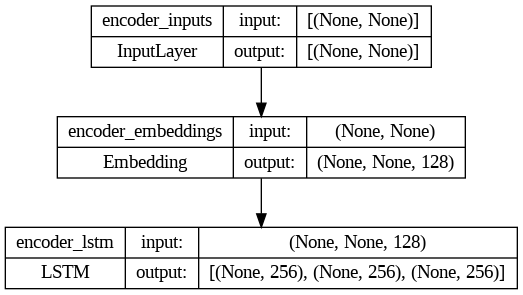
\includegraphics[width=0.5\textwidth]{encoder_model_no_attention_plot.png}
\caption{Visualization of the flow of sequencing in the Encoder}
\end{figure}

\subsection{Decoder}
The decoder is initialized in a similar process where the inputs are its padded training targets, a embedding layer is defined, and an LSTM cell is created. However, when the decoder's embedded inputs are passed through as input for the decoder cell, we pass through the final hidden and context states of the encoder as the initial state of the decoder cell as well to transfer the learned state of the encoder. Lastly, the decoder output sequence, which is the sequence of outputs from the decoder hidden states at each timestamp, is passed through a softmax layer to create a probability distribution of the output word. 
\begin{figure}[h]
\centering
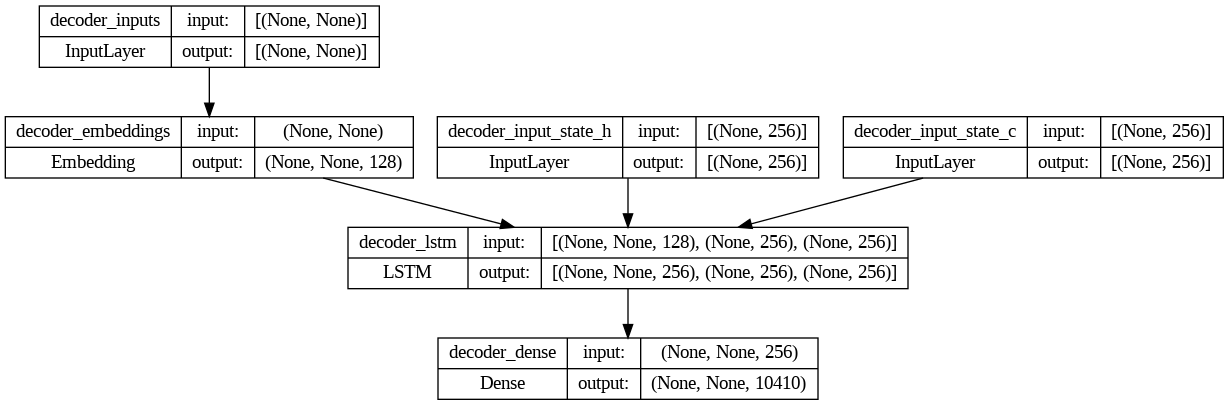
\includegraphics[width=0.5\textwidth]{decoder_model_no_attention_plot.png}
\caption{Visualization of the flow of sequencing in the Decoder}
\end{figure}

\section{Dataset preparation}
The dataset in-use is a .csv file compiling over $100,000$ pairs of English phrases and their translations in Spanish, presumably verified through human judgment. The exact dataset can be downloaded from \nolinkurl{https://www.kaggle.com/datasets/lonnieqin/englishspanish-translation-dataset}. A sample of $95,000$ randomly selected pairs from the set is then split amongst $80\%$ for training, $10\%$ for validation, and $10\%$ for testing.
\section{Plan of Experimental Studies by End of Spring}
As for the timeline for research, roughly a month was spent on testing that the encoder and decoder were operating to expectation with no attention mechanism initially incorporated in order to both ensure that the implementation of the model can be replicated without direction as well as to allot time for deciding the direction of evaluating these models. The rest of the semester should be spent on either testing other attention models or evaluating existing translation data extracted from models tested in this time frame.
\section{Preliminary Results}
Figures $3$-$6$ are diagrams from the notebook of the model with no attention mechanism utilized.
\begin{figure}[h]
    \centering
    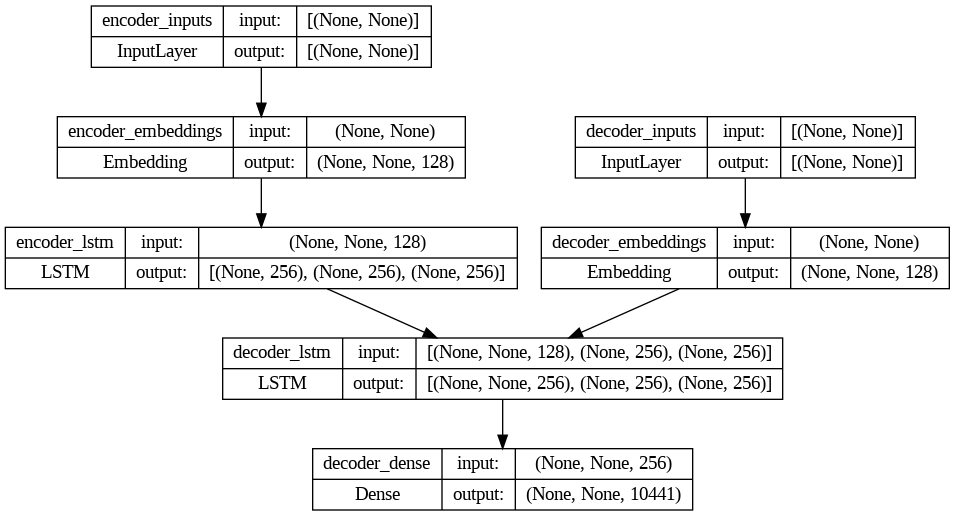
\includegraphics[width=0.5\textwidth]{span_eng_seq2seq_nmt_no_attention.png}
    \caption{Compiled model with no attention mechanism}
\end{figure}
\begin{figure}[h]
    \centering
    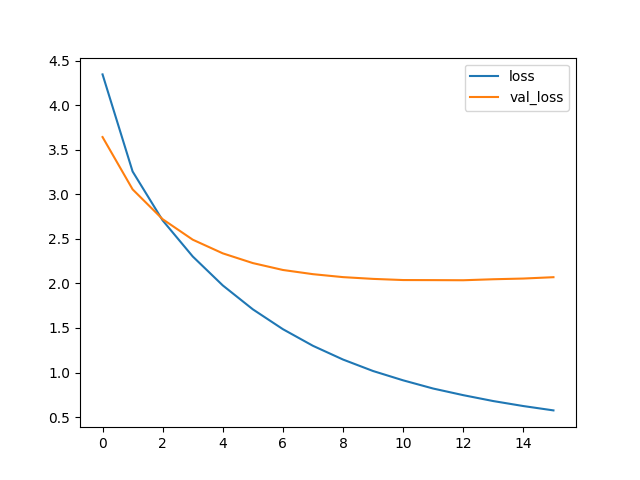
\includegraphics[width=0.5\textwidth]{loss_v_val_loss.png}
    \caption{Loss versus validation loss during model fitting}
\end{figure}
\begin{figure}[h]
    \centering
    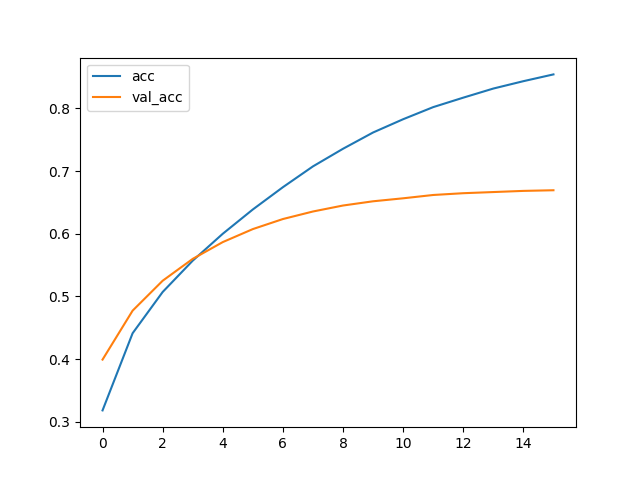
\includegraphics[width=0.5\textwidth]{acc_v_val_acc.png}
    \caption{Model accuracy versus validation accuracy during model fitting}
\end{figure}
\begin{figure}[h]
    \centering
    \includegraphics[width=0.5\textwidth]{sample_translation_evals.png}
    \caption{Evaluation from sample of 10 Spanish phrases translated to English utilizing model with no attention}
\end{figure}

\section{Conclusion}
\subsection{Final Results}
\subsection{}
\medskip

\begin{thebibliography}{00}
\bibitem{b7} Bahdanau, Dzmitry, Kyunghyun Cho, and Yoshua Bengio. "Neural machine translation by jointly learning to align and translate." \textit{arXiv preprint arXiv:1409.0473} (2014).
\bibitem{b13} Brauwers, Gianni, and Flavius Frasincar. "A general survey on attention mechanisms in deep learning." IEEE Transactions on Knowledge and Data Engineering 35.4 (2021): 3279-3298.
\bibitem{b4} Callison-Burch, Chris, Miles Osborne, and Philipp Koehn. "Re-evaluating the role of BLEU in machine translation research." \textit{11th conference of the european chapter of the association for computational linguistics.} 2006.
\bibitem{b12} Choi, Edward, et al. "Retain: An interpretable predictive model for healthcare using reverse time attention mechanism." \textit{Advances in neural information processing systems 29} (2016).
\bibitem{b11} Ghaffarian, Saman, et al. "Effect of attention mechanism in deep learning-based remote sensing image processing: A systematic literature review." \textit{Remote Sensing 13.15} (2021): 2965.
\bibitem{b9} Guo, Meng-Hao, et al. "Attention mechanisms in computer vision: A survey." \textit{Computational visual media 8.3 }(2022): 331-368.
\bibitem{b1} Jones, Karen Sparck. ``Natural language processing: a historical review." \textit{Current issues in computational linguistics: in honour of Don Walker} (1994): 3-16.
\bibitem{b10} Lieskovská, Eva, et al. "A review on speech emotion recognition using deep learning and attention mechanism." \textit{Electronics 10.10} (2021): 1163.
\bibitem{b8} Luong, Minh-Thang, Hieu Pham, and Christopher D. Manning. "Effective approaches to attention-based neural machine translation." arXiv preprint arXiv:1508.04025 (2015).   
\bibitem{b5} Mathur, Nitika, Timothy Baldwin, and Trevor Cohn. "Tangled up in BLEU: Reevaluating the evaluation of automatic machine translation evaluation metrics." \textit{arXiv preprint arXiv:2006.06264} (2020)
\bibitem{b3} Papineni, Kishore, et al. "Bleu: a method for automatic evaluation of machine translation." \textit{Proceedings of the 40th annual meeting of the Association for Computational Linguistics.} 2002.
 \bibitem{b14} Stahlberg, Felix. "Neural machine translation: A review." \textit{Journal of Artificial Intelligence Research 69} (2020): 343-418.

\bibitem{b2} Wu, Lijun, et al. "A study of reinforcement learning for neural machine translation." \textit{arXiv preprint arXiv:1808.08866} (2018).
\bibitem{b6} Zhang, Tianyi, et al. "Bertscore: Evaluating text generation with bert." \textit{arXiv preprint arXiv:1904.09675} (2019).



\end{thebibliography}

\end{document}
